\subsection{DOP 4 Логическое  программирование. Декларативная семантика и операционная семантика;  соотношение между ними.  Стандартная стратегия выполнения логических программ.}

$\mathLet ~ \sigma = \langle Const,Func,Pred\rangle$ — некоторая сигнатура, в которой определяются термы и атомы.

«заголовок» ::= «атом» \\
«тело» ::= «атом» | «тело», «атом» \\ 
«правило» ::= «заголовок» $\leftarrow$ «тело»; \\
«факт» ::= «заголовок»; \\ 
«утверждение» ::= «правило» | «факт» \\ 
«программа» ::= «пусто» | «утверждение» «программа» \\
«запрос» ::= $\square$ | ? «тело» \\

$\mathLet ~ G = ? C_{1},C_{2},\ldots,C_{m}$ — запрос. Тогда
\begin{itemize}
    \item атомы $C_{1},C_{2},\ldots,C_{m}$ называются подцелями запроса G,
    \item переменные множества называются целевыми переменными,
    \item запрос $\square$ называется пустым запросом,
    \item запросы будем также называть целевыми утверждениями.
\end{itemize}
 
\textbf{Полисемантичность} -- одна и та же логическая программа имеет две равноправные семантики, два смысла. \\
Программисту важно понимать, что вычисляет программа. Такое понимание программы называется \textbf{декларативной} семантикой программы. \\ 
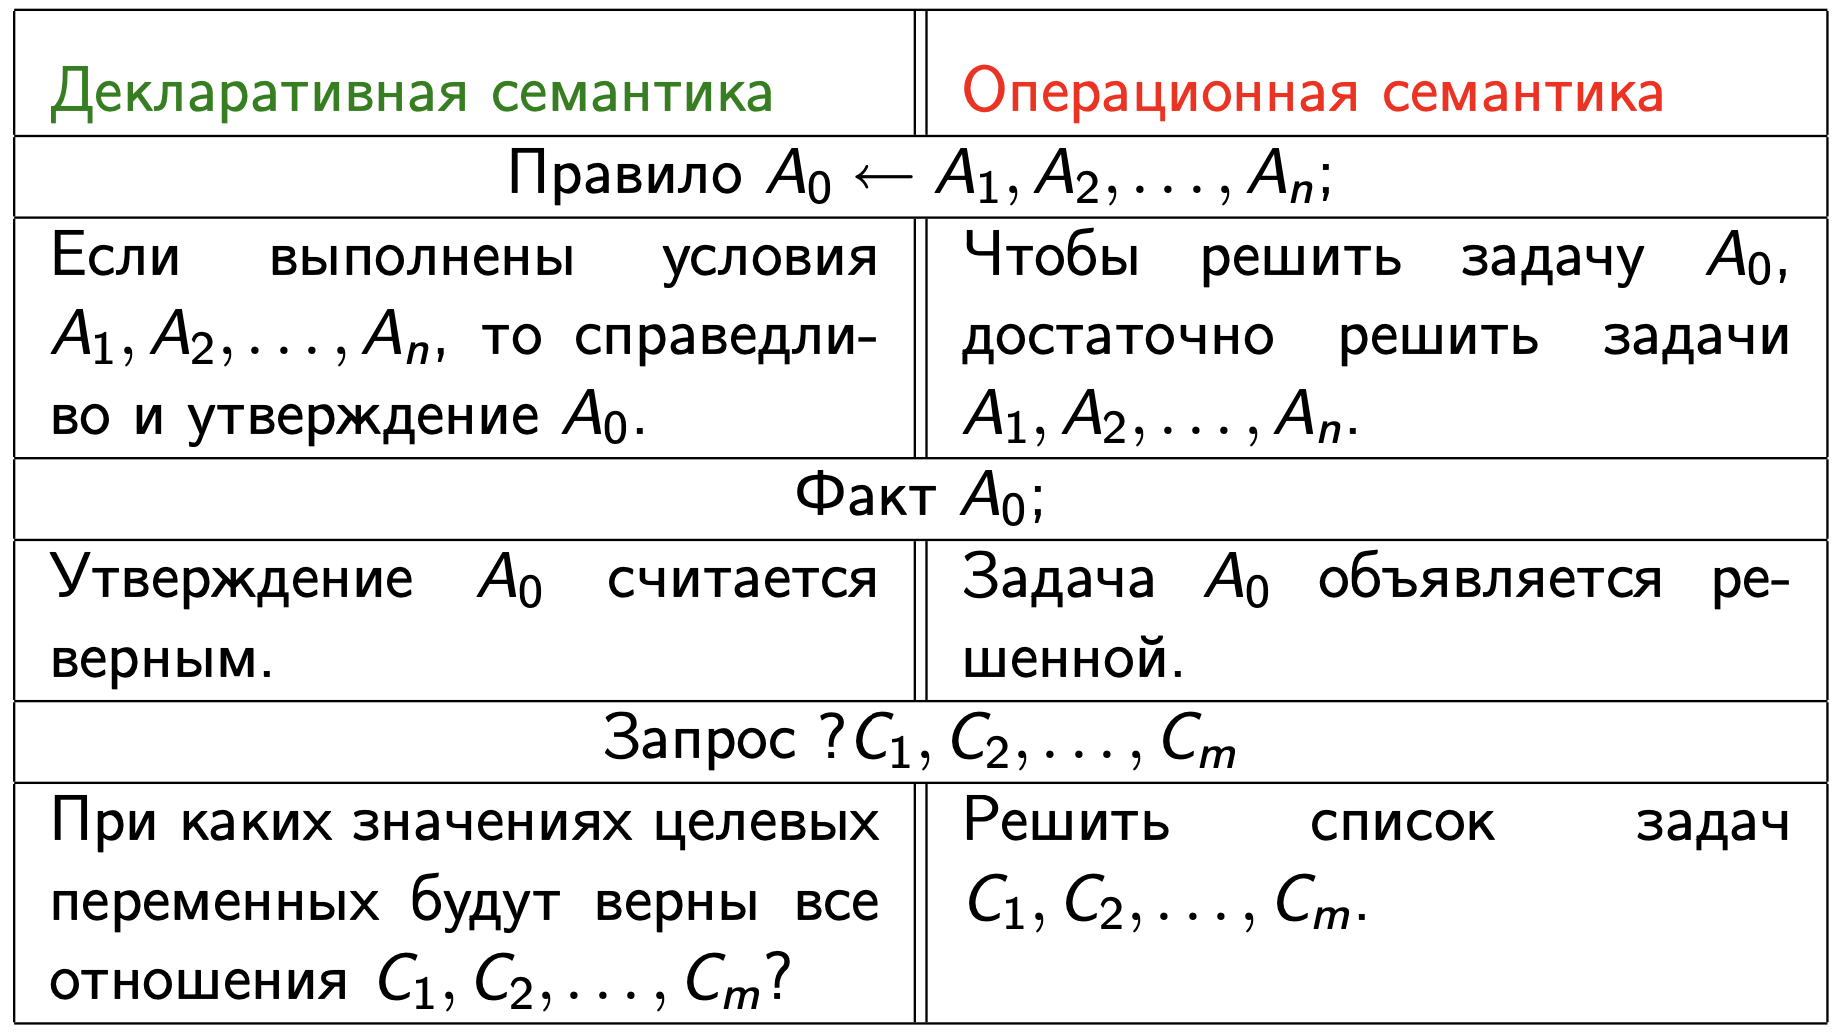
\includegraphics[width=\columnwidth]{pics/comp.png}

С точки зрения декларативной семантики, программные утверждения D и запросы G — это логические формулы, программа P — это множество формул (база знаний), а правильный ответ на запрос — это такие значения переменных (подстановка), при которой запрос оказывается логическим следствием базы знаний.

\mathLet \ P -- логическая программа, G -- запрос к P с множеством целевых переменных $Y_{1},Y_{2},\ldots,Y_{k}$. Тогда всякая подстановка $\theta = \{Y_{1}/t_{1},\ldots,Y_{k}/t_{k}\}$ называется ответом на запрос G к программе P. Ответ $\theta = \{Y_{1}/t_{1},\ldots, Y_{k}/t_{k}\}$ называется \textbf{правильным ответом} на запрос G к программе P, если $P \models \forall Z_{1} \ldots \forall Z_{n}G\theta$, где $\{Z_{1},\ldots,Z_{n}\}$ --- множество свободных переменных в термах $t_i$.

\textbf{Теорема об основном правильном ответе}
$\mathLet ~ G =?C_{1},C_{2},\ldots,C_{m}$ -- запрос к хорновской логической программе P. $\mathLet ~ Y_{1},Y_{2},\ldots,Y_{k}$ — целевые переменные, $t_{1},t_{2},\ldots,t_{k}$ —основные термы.
Тогда подстановка $\theta = \{Y_{1}/t_{1}, \ldots, Y_{k}/t_{k}\}$ является правильным ответом на запрос G к программе P тогда и только тогда, когда $P \models (C_{1} \wedge \ldots \wedge C_{m})\theta$.

Под операционной семантикой понимают правила построения вычислений программы. Компьютеру важно «знать», как проводить вычисление программы. Такое понимание программы называется \textbf{операционной} семантикой программы. Результат работы логической программы --- это правильный ответ на запрос к программе. Значит, операционная семантика должна описывать метод вычисления правильных ответов.

Подстановка $\theta$ -- \textbf{унификатор} выражений $E_1, E_2$, если $E_1 \theta = E_2 \theta$. Подстановка $\theta$ -- \textbf{наиболее общий унификатор (НОУ)} выражений $E_1, E_2$, если $\theta$ -- унификатор выражений $E_1, E_2$ и для любого унификатора $\eta$ существует такая подстановка $\rho$, для которой верно $\eta = \theta \rho$.

Пусть 
\begin{itemize}
    \item $G = ? C_{1},C_{2},\ldots,C_{m}$ — целевое утверждение, в котором выделена подцель $C_{i}$,
    \item $D = A_{0} \leftarrow A_{1},A_{2},\ldots,A_{n}$ —вариант некоторого
программного утверждения, в котором $Var_{G} \cap Var_{D} = 0$,
    \item $\theta \in \text{НОУ}(C_{i},A_{0})$ -- \textbf{наибольший общий унификатор} подцели $C_{i}$ и заголовка программного утверждения $A_{0}$.
\end{itemize}
Тогда запрос 
$P = ?(C_{1},\ldots,C_{i-1}, A_{1} ,A_{2},\ldots,A_{n},C_{i+1},\ldots,C_{i+1},\ldots,C_{m})$ - SLD-резольвентой программного утверждения D и запроса G с выделенной подцелью $C_{i}$ и унификатором $\theta$. 

$\mathLet ~ G = ? C_{1},C_{2},\ldots,C_{m}$ - целевое утверждение, $P = \{D_{1},D_{2},\ldots,D_{m}\}$ - хорновская логическая программа. Тогда частичным SLD-резолютивным вычислением, порожденным запросом $G_{0}$ к логической программе P называется последовательность троек (конечная или бесконечная)\\
$(D_{j_{1}}, \theta_{1}, G_{1}), (D_{j_{2}}, \theta_{2}, G_{2}), \ldots, (D_{n}, \theta_{n}, G_{n}), \ldots$
где 
\begin{itemize}
    \item $D_{ji} \in P, \theta_{i} \in Subst, G_{i}$ — целевое утверждение (запрос);
    \item запрос $G_{i}$ - SLD-резольвента программного утверждения $D_{j_{i}}$ и запроса $G_{i-1}$ с унификатором $\theta_{i}$. 
\end{itemize}
Частичное SLD-резолютивное вычисление \\
$comp = (D_{j_{1}}, \theta_{1}, G_{1}), (D_{j_{2}}, \theta_{2}, G_{2}), \ldots, (D_{n}, \theta_{n}, G_{n})$ называется \textbf{успешным вычислением}, если $G_{n} =\square$, \textbf{бесконечным вычислением}, если comp - это бесконечная последовательность, \textbf{тупиковым вычислением}, если comp - это конечная последовательность, при этом для запроса $G_{n}$ невозможно построить ни одной SLD-резольвенты. 

$\mathLet ~ G = ? C_{1},C_{2},\ldots,C_{m}$ - целевое утверждение с целевыми переменными $Y_{1},Y_{2},\ldots,Y_{k}$, $P = \{D_{1},D_{2},\ldots,D_{m}\}$ --- хорновская логическая программа, $comp = (D_{j_{1}}, \theta_{1}, G_{1}), (D_{j_{2}}, \theta_{2}, G_{2}), \ldots, (D_{n}, \theta_{n}, G_{n})$ - успешное SLD-резолютивное вычисление, порожденное запросом G к программе P. Тогда подстановка $\theta = \{\theta_{1},\theta_{2},\ldots,\theta_{n}\}$, представляющая собой композицию всех вычсиленных унификаторов $\theta_{1},\theta_{2},\ldots,\theta_{n}$, ограниченную целевыми переменными $Y_{1}$,$Y_{2}$,...,$Y_{k}$ называется вычисленным ответом на запрос $G_{0}$ к программе Р. 
У нас есть два типа ответов: 
\begin{itemize}
    \item \textbf{правильные ответы}, которые логически следуют из программы;
    \item \textbf{вычисленные ответы}, которые конструируются по ходу SLD-резолютивных вычислений.
\end{itemize}

\textbf{Теорема корректности операционной семантики относительно декларативной семантики} $\mathLet ~ G = ? C_{1},C_{2},\ldots,C_{m}$ - целевое утверждение, $P = \{D_{1},D_{2},\ldots,D_{m}\}$ - хорновская логическая программа. $\theta$ - вычисленный ответ на вопрос G к программе P. Тогда $\theta$ является правильным ответом на вопрос G к программе P. 

\textbf{Теорема полноты}
$\mathLet ~\theta$ - правильный ответ на вопрос G к хорновской логической программе P. Тогда существует такой вычислительный ответ $\eta$ на запрос G к программе P, что $\theta$=$\eta *p $ для некоторой подстановки p.

Отображение R, которое сопоставляет каждому непустому запросу G = ? $C_{1}$,$C_{2}$,...,$C_{m}$ одну и ту же из подцелей $C_{i}$ = R(G) в этом запросе, называется \textbf{правилом выбора подцелей}. 

Для заданного правила выбора подцелей R вычисление запроса G к логической программе называется \textbf{R-вычислением}, если на каждом шаге вычисления очередная подцель в запросе выбирается по правилу R. 
Ответ, полученный в результате успешного R-вычисления, называется \textbf{R-вычисленным}. 

\textbf{Теорема сильной полноты} Каково бы ни было правило выбора подцелей R, если $\theta$ - правильный ответ на запрос G к хорновской логической программе P, то существует такой R-вычисленный ответ $\eta$, что равенство $\theta = \eta$р. 

\textbf{Деревом SLD-резолютивных вычислений} запроса G к логической программе P называется помеченное корневое дерево $T_{G,P}$, удовлетворяющее следующим требованиям: 
\begin{itemize}
    \item Корнем дерева является исходный запрос G.
    \item Потомками аждой вершины G являются всевозможные SLD-резольвенты запроса G.  
    \item Листовыми вершинами вляются пустые запросы и запросы, не имеющие SLD-резольвент. 
\end{itemize}

\textbf{Стратегией вычисления запросов} к логическим программам называется алгоритм построения (обхода) дерева SLD-резолютивных вычислений всякого запроса G к произвольной логической программе P.

Стратегия вычислений называется \textbf{вычислительно полной} , если для любого запроса G и любой логической программы P эта стратегия строит (обнаруживает) все успешные вычисления запроса G к программы P. 

\textbf{Стратегия обхода в ширину}: дерево строится (обходится) поярусно --- вершина i-го яруса не строится, до тех пор пока не будут построены все вершины $(i - 1)$-го яруса. Эта стратегия является полной, но вычислительно затратной.

\textbf{Стратегия обхода в глубину с возвратом}: ветви дерева обходятся поочередно (слева направо) — очередная ветвь дерева не обходится, до тех пор пока не будут пройдены все вершины текущей ветви. Не является полной, но быстрая. Она и является стандартной стратегией выполнения логических программ.

% -------- source --------
\bigbreak
[\cite[page 69-96]{replace_me}]